\section{VL 12: Kontexte sind verzahnt: Social Media}

\textbf{Web 2.0}, das Web wird als Plattform benutzt, auf der alle Benutzer Inhalte
gemeinsam verändern und hinzufügen.

\textbf{Social Media}, eine Gruppe von Webanwendungen, die auf Web 2.0 aufbauend
den Nutzern \emph{Herstellung} und \emph{Austausch} digitaler Inhalte (\emph{User
Generated Content}) ermöglichen.

\begin{itemize}
\item Peer-to-Peer Kommunikation
\item User Generated Content
\item Einfachheit der Nutzung
\item Hohe Verfügbarkeit (jeder, überall, jederzeit)
\item Öffentliche Handlungen
\end{itemize}

\textbf{Früher} (Web 1.0): IT hat Geschäftsprozesse ermöglicht und angetrieben

\textbf{Heute} (Web 2.0): Hohe Nutzerzahlen treiben den Fortschritt an, IT setzt um.

\subsection{Anwendungsklassen von Social Media}

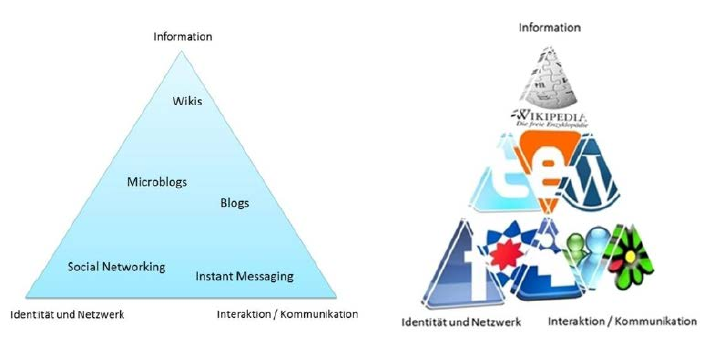
\includegraphics[width=0.9\textwidth]{anwendungsklassen.png}

Einteilung: Private (Facebook etc.) / Business/Professional (LinkedIn...) / Specialized (Github!)

\subsection{Enterprise 2.0}

Enterprise 2.0 ist die Nutzung von Social Media entweder \emph{innerhalb einer
Organisation} oder \emph{als Verbindung zu Partnern und Kunden} $\Rightarrow$ offene
Innen- und Außenkommunikation.

\textbf{Interne Nutzung}: Zusammenarbeit, Austausch von Wissen, Verbesserung von Prozessen.

\textbf{Externe Nutzung}: Marketing, Imagebildung, Recruiting, Zusammenarbeit mit Experten / Zulieferern.
\newpage
